\documentclass{exam}
\usepackage{xcolor, minted, graphicx, fontspec}
\setmainfont{Open Sans}
\graphicspath{ {./images} }

\author{Jordy Alkema}
\title {Homework Week 2}

\begin{document}
\maketitle

\section{Review}
\begin{questions}
	\question
	\begin{parts}
		\part
		5, 1 voor elk van de volgende tables: test, unit of measure, variable, sample, organization
		\part
		Ik zou de tabel opsplitsen in een overkoepelende tabel voor observation met: date, time en value en twee tabellen voor physical observations en test observations, om zo op de volgende structuur uit te komen.

		\textbf{observation:}
		\begin{itemize}
			\item id (PK)
			\item unit (FK)
			\item variable (FK)
			\item party (FK)
			\item date
			\item time
			\item value
		\end{itemize}
		\textbf{test\_observation}
		\begin{itemize}
			\item id (PK)
			\item observation (FK)
			\item test (FK)
		\end{itemize}
		\textbf{physical\_observation}
		\begin{itemize}
			\item id (PK)
			\item observation (FK)
			\item sample (FK)
		\end{itemize}
		\part
		De volgende waarden zijn een record voor een physical observation

		\begin{center}
			\textbf{observation:}

			\begin{tabular}{ | c | c | c | c | c | c | c |}
				\hline
				id & unit & variable & party & date       & time  & value \\
				\hline
				1  & 1    & 1        & 1     & 08-03-2023 & 12:00 & 7     \\
				\hline
			\end{tabular}

			\textbf{physical\_observation}

			\begin{tabular}{ | c | c | c | }
				\hline
				id & observation & sample \\
				\hline
				1  & 1           & 1      \\
				\hline
			\end{tabular}
		\end{center}
	\end{parts}
	\pagebreak
\end{questions}

\section{Questions}
\begin{questions}
	\question
	\begin{parts}
		\part
		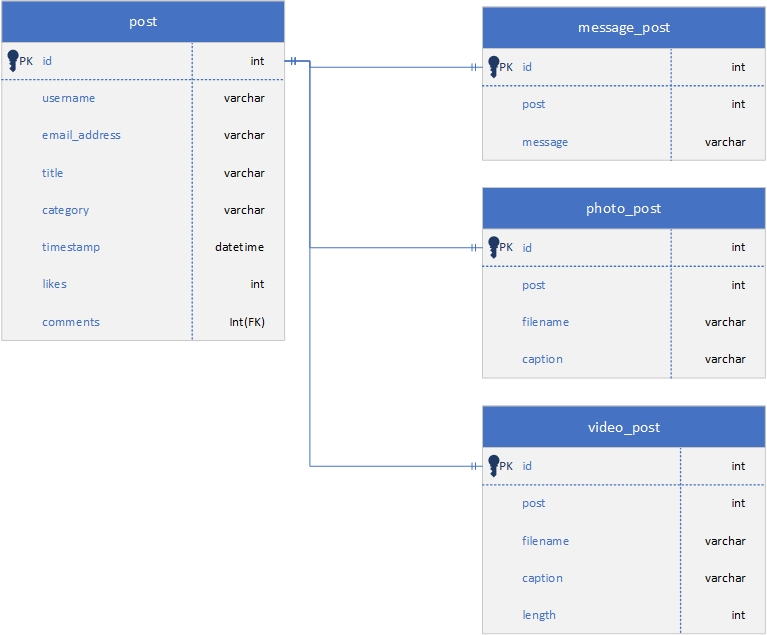
\includegraphics[width=\textwidth,height=\textheight,keepaspectratio]{question2a}
	\end{parts}
\end{questions}

\end{document}
